% !TeX root = ../libro.tex
% !TeX encoding = utf8

\setchapterpreamble[c][0.75\linewidth]{%
	\sffamily
	En este capítulo abordaremos algunos algoritmos de búsqueda en grafos, con el objetivo de encontrar caminos entre puntos, geodésicas y componentes conexas asociadas a los distintos grafos. En esta sección nos referiremos a los vértices del grafo por nodos.
	\par\bigskip
}
\chapter{Algoritmos de búsqueda en grafos}\label{ch:tercer-capitulo}

\section{Algoritmo de búsqueda en anchura}

El algoritmo de búsqueda en anchura (BFS-Breadth First Search en inglés) es un algoritmo de búsqueda no informada, es decir, que cuando se da un paso en el algoritmo, no se sabe si este es el mejor posible. Es uno de los algoritmos más simples de búsqueda en grafos y funciona como base para el desarrollo de otros algoritmos más complejos. La idea intuitiva del algoritmo es partir del nodo inicial e ir explorando todos los nodos vecinos (conectados mediante un camino), cuando se han explorado todos los vecinos, se repite el proceso para cada uno de estos, hasta recorrer todo el grafo. \\

El nombre de búsqueda en anchura viene del hecho de que el algoritmo explora la frontera entre nodos explorados y no explorados, de manera uniforme a lo largo del ancho de la misma, es decir, explora todos los nodos a distancia $k$ antes de explorar un nodo a distancia $k+1$. \\

El algoritmo funciona tanto en grafos no dirigidos como grafos dirigidos, sin embargo, requiere que los pesos de las aristas sean $1$, es decir, que sea un grafo no ponderado. El algoritmo se puede utilizar tanto para calcular las componentes conexas de un grafo como para encontrar los caminos de mínima longitud, geodésicas, entre dos nodos. \\

Desde un punto de vista matemático, sea $p$ el nodo inicial, el algoritmo consiste en explorar la bola cerrada $\overline B_p(r)$ empezando en $r=1$, marcando los elementos dentro de la bola, e ir aumentando en cada paso el radio en una unidad hasta que no se puedan alcanzar más elementos desde el nodo inicial, es decir, hasta que $\overline B_p(r)\cap \overline B_p(r+1) = \emptyset$. Para el cálculo de componentes conexas, si, tras terminar el proceso anterior, quedan nodos sin explorar, se selecciona un nodo no explorado y se repite el proceso, hasta que todos los nodos sean explorados. Para el cálculo de las geodésicas la exploración continúa hasta encontrar el nodo destino, si no se encuentra, no existe camino entre los nodos.

\begin{proposicion}\label{prop:BFS}
	\textbf{(Corrección del algoritmo de búsqueda en anchura)} Sea $v \in V$ el nodo inicial y $p \in V$ el nodo final, el camino encontrado por el algoritmo de búsqueda en anchura entre estos nodos es una geodésica.
\end{proposicion}

\begin{proof}
	Sea $l$ la longitud del camino encontrado, por construcción del algoritmo, esto supone dos cosas, por un lado, $p \in \overline B_v(l)$, y, por otro lado, $p \notin \overline B_v(r)\ \forall r<l$ pues, de lo contrario, el algoritmo hubiera parado antes de explorar $\overline B_v(l)$ y la longitud sería menor. Pero entonces esto supone que no existe ningún camino entre $v$ y $p$ de longitud menor que $l$, es decir, que el camino encontrado de longitud $l$ es una geodésica, como se quería.
\end{proof}


\begin{figure}[htb]
	\centering
	\begin{subfigure}{0.25\linewidth}
		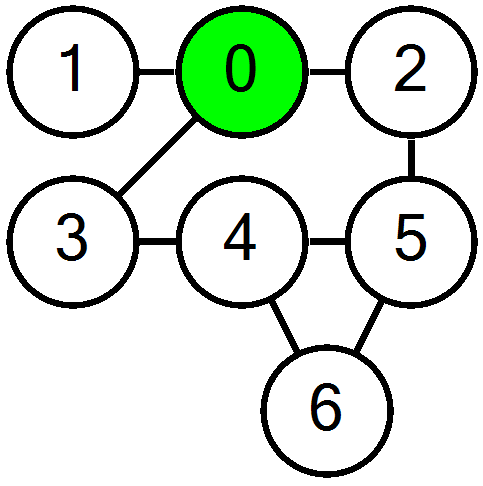
\includegraphics[width=\linewidth]{BFS/graf-bfs-camino-1}
		\caption{}
	\end{subfigure}
	\begin{subfigure}{0.25\linewidth}
		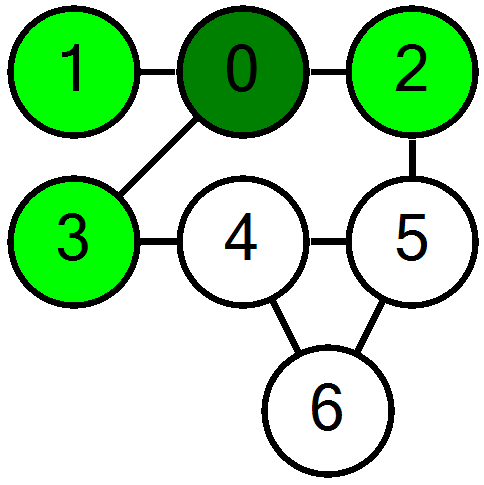
\includegraphics[width=\linewidth]{BFS/graf-bfs-camino-2}
		\caption{}
	\end{subfigure}
	\begin{subfigure}{0.25\linewidth}
		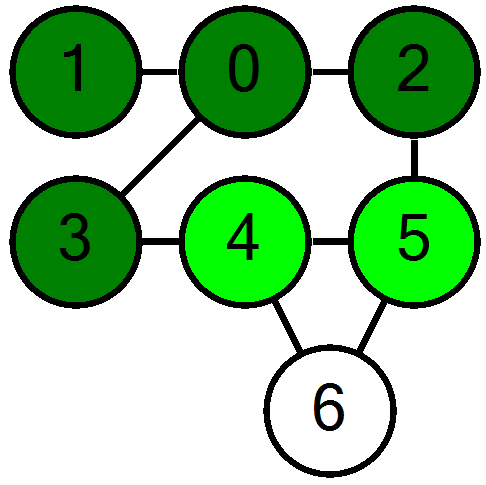
\includegraphics[width=\linewidth]{BFS/graf-bfs-camino-3}
		\caption{}
	\end{subfigure}
	\begin{subfigure}{0.25\linewidth}
		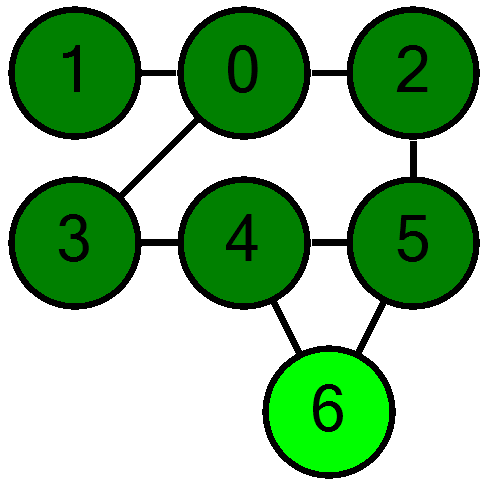
\includegraphics[width=\linewidth]{BFS/graf-bfs-camino-4}
		\caption{}
	\end{subfigure}
	\begin{subfigure}{0.25\linewidth}
		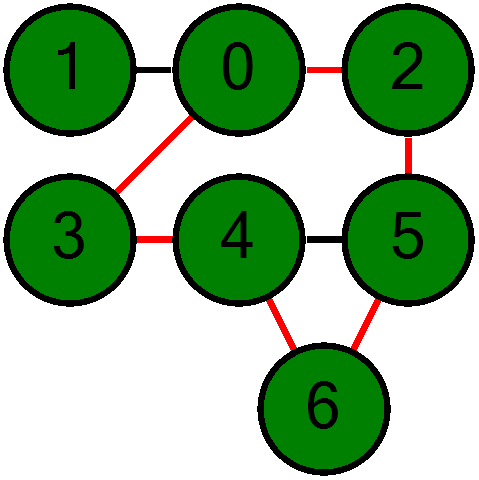
\includegraphics[width=\linewidth]{BFS/graf-bfs-camino-5}
		\caption{}
	\end{subfigure}
	\caption{Cálculo de las geodésicas entre el nodo $0$ y el nodo $6$.}
	\label{fig:bfs-camino}
\end{figure}

\begin{figure}[!]
	\centering
	\begin{subfigure}{0.25\linewidth}
		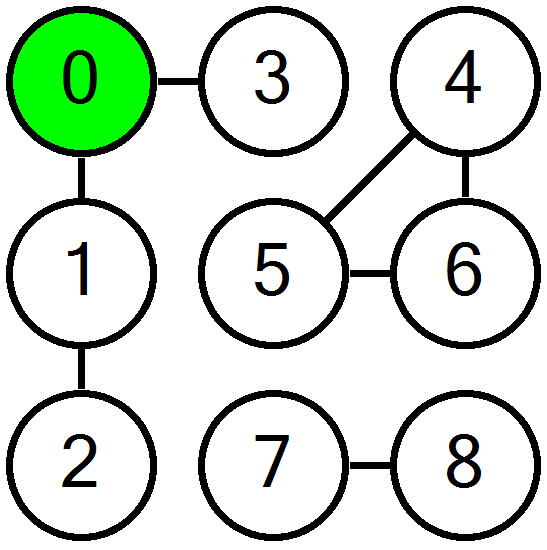
\includegraphics[width=\linewidth]{BFS/graf-bfs-conexas-1}
		\caption{}
	\end{subfigure}
	\begin{subfigure}{0.25\linewidth}
		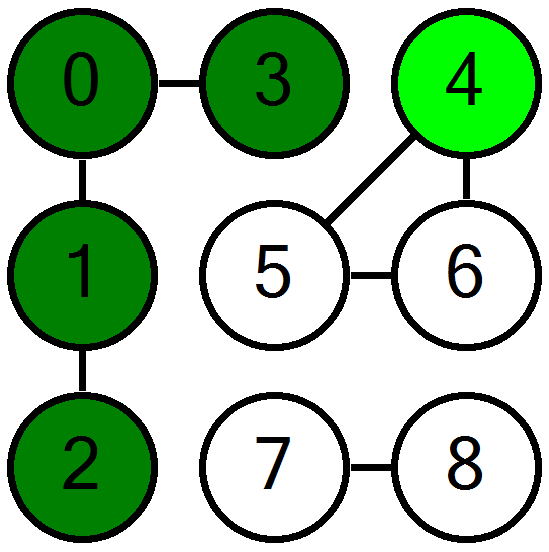
\includegraphics[width=\linewidth]{BFS/graf-bfs-conexas-2}
		\caption{}
	\end{subfigure}
	\begin{subfigure}{0.25\linewidth}
		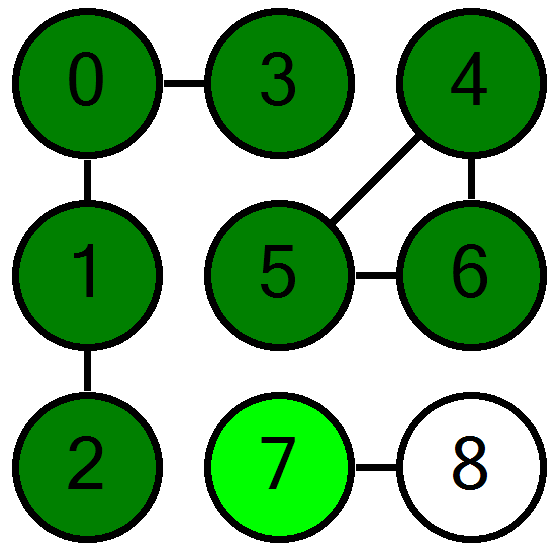
\includegraphics[width=\linewidth]{BFS/graf-bfs-conexas-3}
		\caption{}
	\end{subfigure}
	\begin{subfigure}{0.25\linewidth}
		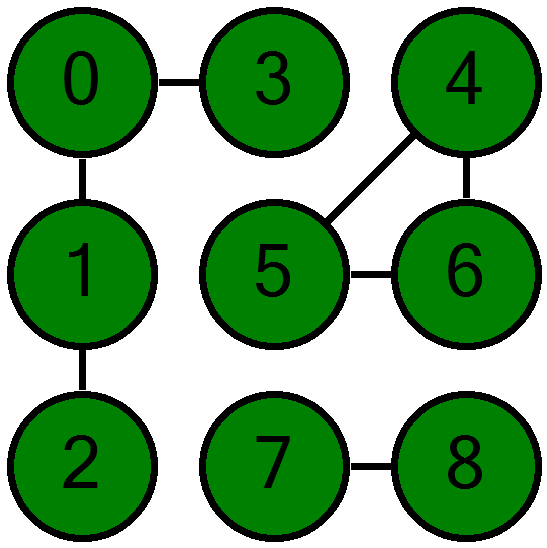
\includegraphics[width=\linewidth]{BFS/graf-bfs-conexas-4}
		\caption{}
	\end{subfigure}
	\caption{Cálculo de las componentes conexas del grafo, en este caso, 3.}
	\label{fig:bfs-conexas}
\end{figure}

En la \autoref{fig:bfs-camino} y la \autoref{fig:bfs-conexas} podemos observar un ejemplo del comportamiento del algoritmo, tanto para encontrar las geodésicas entre dos nodos como para calcular el número de componentes conexas. En el primer caso, se muestra en cada figura el estado de los nodos tras la exploración completa de cada bola, marcando en verde oscuro los nodos explorados y en verde pistacho los nodos visitados que serán explorados en la siguiente bola, por ejemplo, en el apartado (c) acaba de finalizar la exploración de la bola $\overline B_0(1)$. En la segundo figura se muestra el estado del grafo tras finalizar el algoritmo base sobre cada componente, y haber seleccionado el siguiente nodo a explorar.


\subsection{Implementación del algoritmo de búsqueda en anchura}
A continuación veremos la implementación mediante pseudocódigo de las dos versiones del algoritmo que trabajaremos, la primera, cuya finalidad será la de encontrar todas las geodésicas entre dos nodos, y la segunda, que calculará el número de componentes conexas del grafo. \\

Para la construcción del algoritmo, utilizaremos la representación mediante listas de adyacencia. \\

Empezamos por el algoritmo de cálculo de geodésicas entre dos nodos.

\begin{algorithm}
	\caption{BFS\_geodesicas(G, v, p)}
	\begin{algorithmic}[1]
		\For{$u \in G.V$}
			\State $u.explorado = False$
			\State $u.distancia = \infty$
			\State $u.predecesor = \{\}$
		\EndFor
		\State $v.distancia = 0$
		\State $Cola\ Q = \emptyset$
		\State $Q.push(v)$
		\While{$Q \neq \emptyset$}
			\State $u = Q.pull()$
			\If{$u == p$}
				\Return $TRUE$
			\EndIf
			\For{$n \in G.Adj[u]$}
				\If{$!n.explorado$}
					\If{$n.distancia >= u.distancia + 1$}
						\State $n.distancia = u.distancia + 1$
						\State $n.predecesor.push(u)$
						\State $Q.push(n)$
					\EndIf
				\EndIf
			\EndFor
			\State $u.explorado = True$
		\EndWhile
		\Return $FALSE$
	\end{algorithmic}
\end{algorithm}

En el algoritmo anterior, $G$ es el grafo, $v$ el nodo inicial, $p$ el nodo final y $Q$ es una cola. \\

Esta versión del algoritmo es muy similar a la versión normal del algoritmo, con la excepción de que, para poder encontrar todas las geodésicas, debemos considerar nodos ya visitados, pues pueden ser explorados por varios nodos a la misma distancia. Para evitar que antes de explorar un nodo sea visitado y, por tanto, alterado, por otro nodo a distancia mayor que la primera vez que fue visitado, se ha incluido el condicional de la línea 13, nótese que, al iniciar las distancias a infinito, la primera vez que se visita un nodo, este condicional es siempre cierto. \\

Pasamos a continuación con la versión del algoritmo que calcula el número de componentes conexas del grafo.

\begin{breakablealgorithm}
	\caption{BFS\_conexas(G)}
	\begin{algorithmic}[1]
		\State $N = \emptyset$
		\State $conexas = 0$
		\For{$u \in G.V$}
			\State $u.explorado = False$
			\State $N.push(u)$
		\EndFor
		\While{$N \neq \emptyset$}
			\State $conexas = conexas + 1$
			\State $u = N.pull()$
			\State $u.explorado = True$
			\State $Cola\ Q = \emptyset$
			\State $Q.push(u)$		
			\While{$Q \neq \emptyset$}
				\State $u = Q.pull()$
				\For{$n \in G.Adj[u]$}
					\If{$!n.explorado$}
						\State $Q.push(n)$
						\State $n.explorado = True$
						\State $N.remove(n)$
					\EndIf
				\EndFor
			\EndWhile
		\EndWhile
		\Return $conexas$
	\end{algorithmic}
\end{breakablealgorithm}

Para asegurarnos de que se exploran todos los nodos, los incluimos primero en un conjunto, del que los sacamos conforme los exploramos, y continuamos explorando hasta que dicho conjunto sea vacío. Puesto que, para el cálculo de las componentes conexas tan solo necesitamos conocer si podemos alcanzar un nodo desde el inicio, marcamos como explorado los nodos en la adyacencia del nodo que estamos explorando, de tal manera nos aseguramos que solo entra a la cola una vez. 

\section{Algoritmo de Dijkstra}

El siguiente algoritmo que vamos a estudiar es el algoritmo de Dijkstra, al igual que la búsqueda en anchura, es un algoritmo de búsqueda del camino más corto entre nodos, con la salvedad de que funciona también para grafos ponderados. Su nombre proviene del científico Edsger Dijkstra, que lo ideó en 1956 y publicó por primera vez en 1959. \\

La idea del algoritmo es en esencia, la misma que la búsqueda en anchura, con la salvedad de que la exploración de los nodos se realiza de forma ordenada, es decir, en cada paso, se escoge el nodo que esté a distancia menor de todos los que han sido visitados, para explorar. Al igual que el algoritmo de búsqueda en anchura, este algoritmo no funciona si existen aristas con pesos negativos. \\

A nivel de espacios métricos, sea $p$ el nodo inicial, el primer paso es calcular el mínimo de las distancias del resto de nodos a $p$, sea $r$ dicha distancia, entonces procederemos a explorar la bola cerrada $\overline B_p(r)$, en dicha bola se encuentran el nodo inicial y, al menos, un nodo más, que está a distancia r. El siguiente paso es calcular $r'$, que va a ser el mínimo entre las distancias de los nodos no explorados a $p$, y las distancias de los nodos no explorados a los nodos del conjunto $\overline B_p(r)\backslash\{p\}$ más la distancia de dichos nodos a $p$, es decir:

$$r' = min\{d(p,v):\ v \in V\backslash\overline B_p(r),\ d(p,v) + d(v,u):\ v \in \overline B_p(r)\backslash\{p\},\ u \in V\backslash\overline B_p(r)\}$$

A continuación se explora la bola cerrada $\overline B_p(r')$ y el proceso se repite hasta encontrar el nodo destino.

\begin{proposicion}\label{prop:DJK}
	\textbf{(Corrección del algoritmo de Dijkstra)}Sea $v \in V$ el nodo inicial y $p \in V$ el nodo final, el camino encontrado por el algoritmo de Dijkstra entre estos nodos es una geodésica.
\end{proposicion}

\begin{proof}
	Puesto que $d(p,v) > r,\ v \in V\backslash\overline B_p(r)$, por elección de $r$, y $d(p,v) + d(v,u) > r,\ v \in \overline B_p(r)\backslash\{p\},\ u \in V\backslash\overline B_p(r)$, pues, de lo contrario, $d(p,u) \leq d(p,v) + d(v,u) \leq r$, pero esto significa que $u \in \overline B_p(r)$, lo que es una contradicción. Por tanto, se verifica que, en cada paso del algoritmo, $r' > r$, es decir, que la distancia de los nodos explorados es siempre creciente, por lo que la demostración de la \autoref{prop:BFS} es cierta también para este algoritmo.
\end{proof}

\subsection{Implementación del algoritmo de Dijkstra}

A nivel de implementación el algoritmo difiere un poco de la definición matemática, pues es muy ineficiente tener que actualizar el radio en cada paso, teniendo en cuenta además todos los nodos del grafo. Por esto, se introduce el concepto de nodos \textit{visitados}, que son los nodos vecinos de un nodo explorado, es decir, nodos en la frontera del conjunto de nodos explorados. Se introduce este concepto pues, tras la exploración de un nodo, el siguiente nodo que escoge el algoritmo es el de menor distancia y éste es siempre un nodo en la frontera, es decir, un nodo marcado como visitado, pues el resto de nodos del grafo están a mayor distancia de los nodos en la frontera, ya que los pesos de las aristas son positivos. \\

El procedimiento del algoritmo entonces consiste en explorar el nodo visitado a menor distancia del nodo inicial. La exploración del nodo consiste en marcar todos los nodos vecinos no explorados como visitados y actualizar su distancia al nodo inicial a partir del peso de la arista que los une y la distancia del propio nodo. \\

Este procedimiento mantiene invariante la propiedad principal del algoritmo, la distancia de los nodos explorados es siempre creciente a medida que avanza el algoritmo, lo que permite mantener la corrección del algoritmo probada en la \autoref{prop:DJK}, es decir, lo caminos encontrados de esta manera son geodésicas. \\

\begin{figure}[htb]
	\centering
	\begin{subfigure}{0.32\linewidth}
		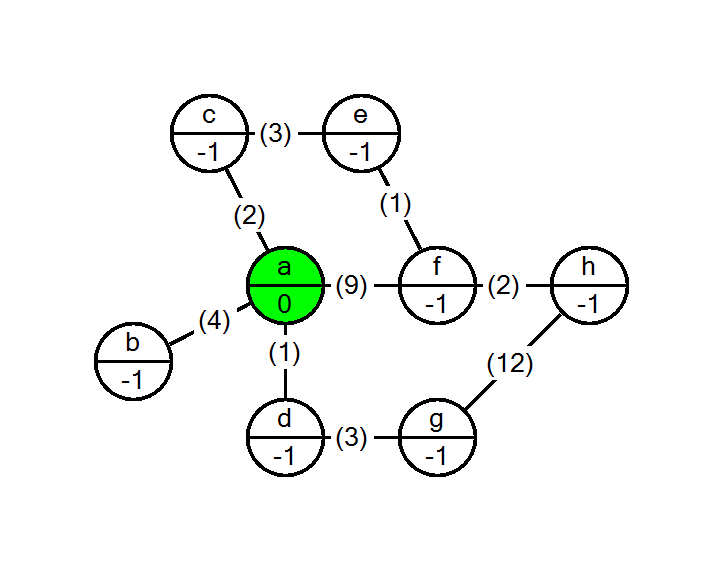
\includegraphics[width=\linewidth]{DJK/graf-djk-1}
		\caption{}
	\end{subfigure}
	\begin{subfigure}{0.32\linewidth}
		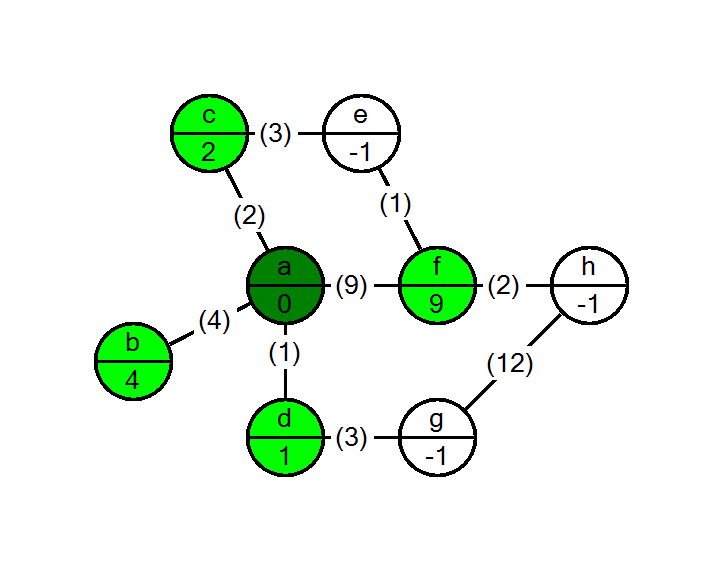
\includegraphics[width=\linewidth]{DJK/graf-djk-2}
		\caption{}
	\end{subfigure}
	\begin{subfigure}{0.32\linewidth}
		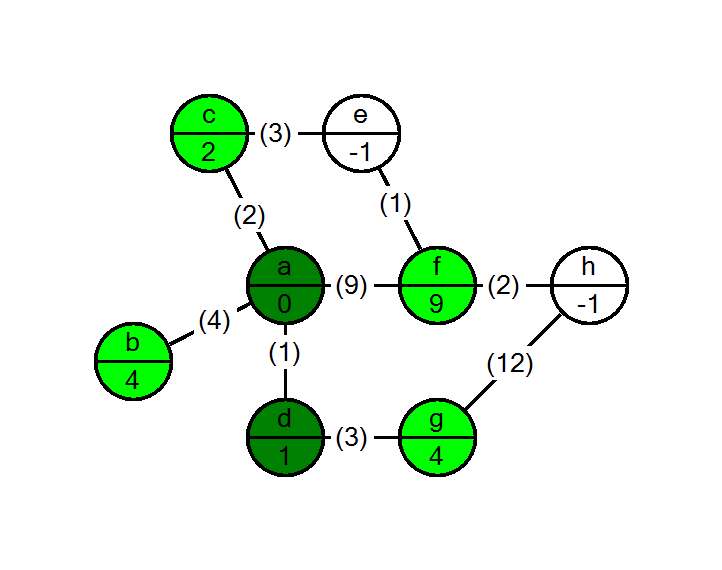
\includegraphics[width=\linewidth]{DJK/graf-djk-3}
		\caption{}
	\end{subfigure}
	\begin{subfigure}{0.32\linewidth}
		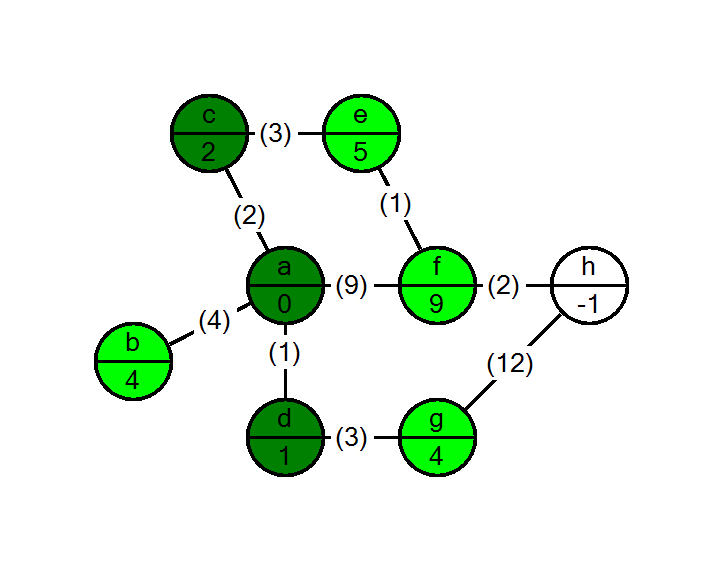
\includegraphics[width=\linewidth]{DJK/graf-djk-4}
		\caption{}
	\end{subfigure}
	\begin{subfigure}{0.32\linewidth}
		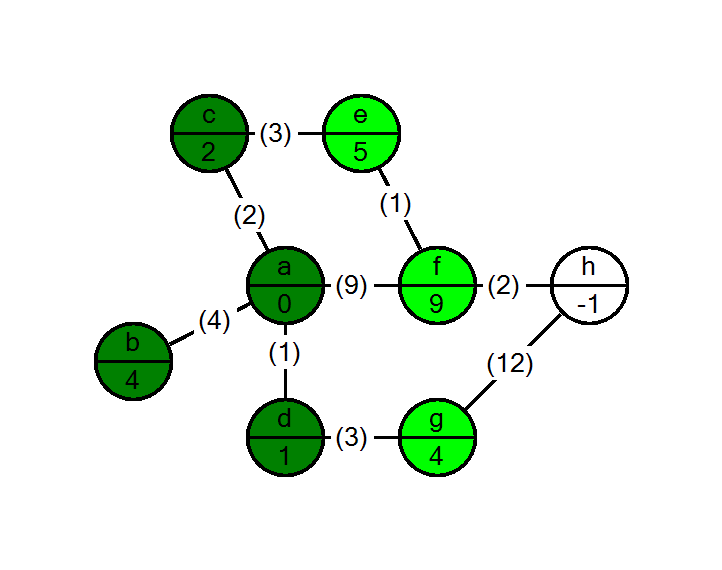
\includegraphics[width=\linewidth]{DJK/graf-djk-5}
		\caption{}
	\end{subfigure}
	\begin{subfigure}{0.32\linewidth}
		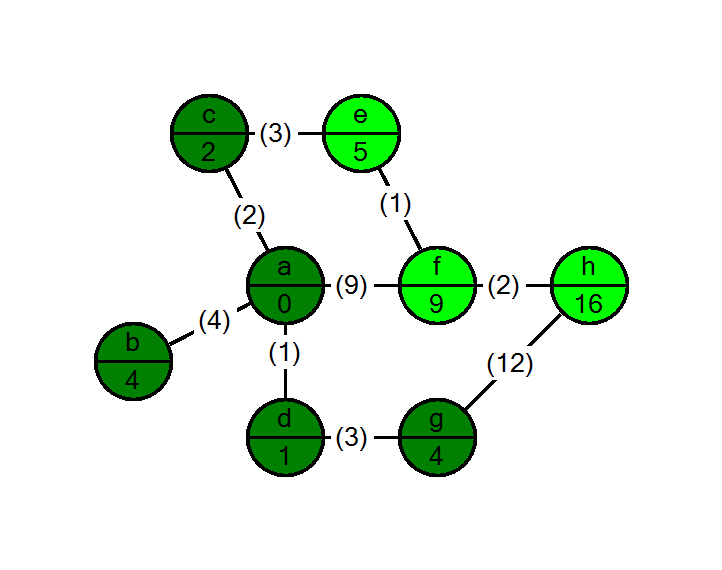
\includegraphics[width=\linewidth]{DJK/graf-djk-6}
		\caption{}
	\end{subfigure}
	\begin{subfigure}{0.32\linewidth}
		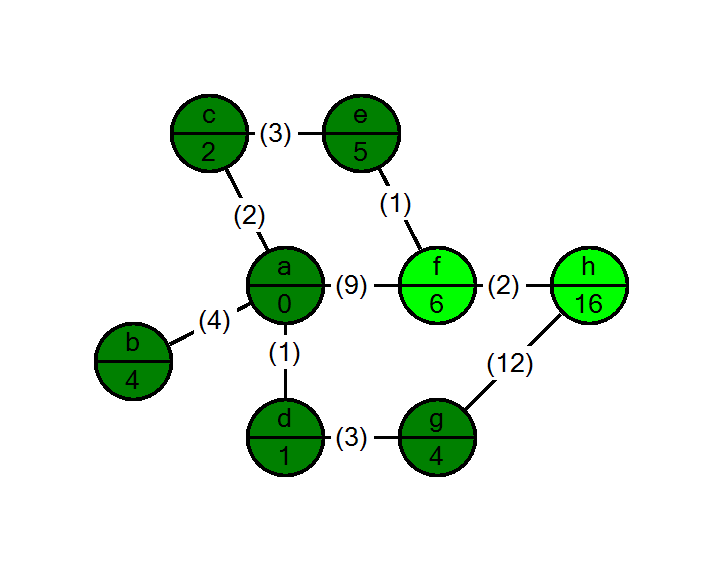
\includegraphics[width=\linewidth]{DJK/graf-djk-7}
		\caption{}
	\end{subfigure}
	\begin{subfigure}{0.32\linewidth}
		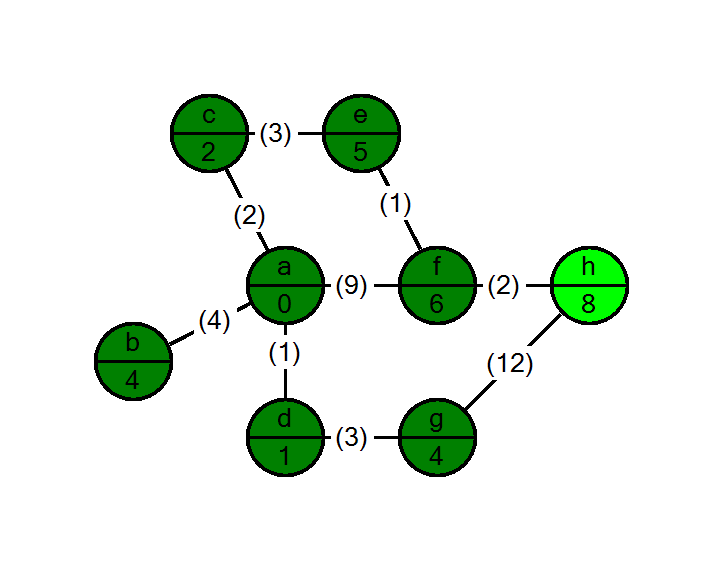
\includegraphics[width=\linewidth]{DJK/graf-djk-8}
		\caption{}
	\end{subfigure}
	\begin{subfigure}{0.32\linewidth}
		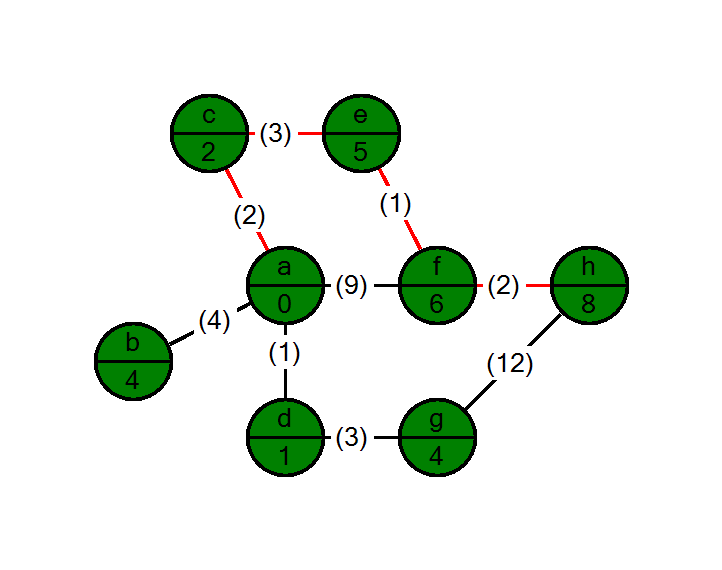
\includegraphics[width=\linewidth]{DJK/graf-djk-9}
		\caption{}
	\end{subfigure}
	\caption{Cálculo de las geodésicas entre el nodo $a$ y el nodo $h$.}
	\label{fig:djk}
\end{figure}

En la \autoref{fig:djk} se puede observar un ejemplo del algoritmo, se empieza marcando el nodo inicial, $a$, como visitado, con distancia $0$, y el resto de nodos con distancia $-1$, para señalar que no han sido visitados todavía. A continuación se escoge el nodo visitado (en verde pistacho) con menor distancia y se explora, es decir, se marcan todos sus vecinos no explorados y no visitados como visitados y se actualizan las distancias de dichos nodos como la distancia del propio nodo más el peso de la arista que los une. En caso de que un nodo vecino esté marcado como visitado, si la distancia desde el nodo actual es menor a la distancia guardada, se actualiza, como se puede observar en el apartado (g). El algoritmo termina cuando se explora el nodo final o no quedan nodos visitados que explorar. \\


Este comportamiento se puede simular utilizando una cola con prioridad en el algoritmo BFS en vez de una cola normal, de tal manera que el nodo escogido en cada paso sea el de menor distancia. \\

Se muestra a continuación el pseudocódigo asociado a la implementación del algoritmo.

\begin{breakablealgorithm}
	\caption{DJK\_geodesicas(G, v, p)}
	\begin{algorithmic}[1]
		\For{$u \in G.V$}
			\State $u.explorado = False$
			\State $u.distancia = \infty$
			\State $u.predecesor = \{\}$
		\EndFor
		\State $v.distancia = 0$
		\State $Cola\ con\ prioridad\ Q = \emptyset$
		\State $Q.push(v)$
		\While{$Q \neq \emptyset$}
			\State $u = Q.pull()$
			\If{$u == p$}
				\Return $TRUE$
			\EndIf
			\For{$n \in G.Adj[u]$}
				\If{$!n.explorado$}
					\If{$n.distancia > u.distancia + d[u][n]$}
						\State $n.distancia = u.distancia + d[u][n]$
						\State $n.predecesor = \{u\}$
						\State $Q.push(n)$
					\ElsIf{$n.distancia == u.distancia + d[u][n]$}
						\State $n.predecesor.push(u)$
					\EndIf
				\EndIf
			\EndFor
			\State $u.explorado = True$
		\EndWhile
		\Return $FALSE$
	\end{algorithmic}
\end{breakablealgorithm}

En el algoritmo anterior, $G$ es el grafo, $v$ el nodo inicial, $p$ el nodo final, $Q$ una cola con prioridad y los pesos de las aristas vienen dados en una matriz, donde el valor $d[a][b]$ corresponde al peso de la arista que une $a$ con $b$.

\section{Algoritmo de Bellman-Ford}

A continuación estudiaremos el algoritmo de Bellman-Ford, que introduce una mejora a los algoritmos anteriores al ser capaz, no sólo de funcionar con grafos con pesos negativos, si no también de detectar la existencia de ciclos negativos en un grafo, situación en la cual el camino de longitud mínima no está bien definida, pues, podríamos entrar en el ciclo negativo y reducir el coste de cualquier camino todo lo que quisiéramos. \\

Este algoritmo resuelve un problema similar al del cálculo de geodésicas entre dos nodos pero con una ligera diferencia, en este caso se calculan las geodésicas desde el nodo inicial a cualquier otro nodo del grafo. \\

Si queremos conocer las geodésicas entre dos nodos concretos, ejecutamos el algoritmo con el nodo inicial y, tras terminar, recuperamos las geodésicas a través de los padres del nodo final. \\

A partir de esta operación, el algoritmo consiste en realizar $|V|-1$ relajaciones de todas las aristas del grafo, es decir, se relajan todas las aristas del grafo y, a continuación, se repite el proceso $|V|-1$ veces. Tras esto, se comprueba la condición de relajación para cada arista, y, en caso de existir alguna arista que la cumpla, esto significa que existe un ciclo negativo y el algoritmo termina con valor $FALSE$. En caso contrario, el algoritmo termina con valor $TRUE$. \\

\begin{lema}\label{lema:corr_Bell_Ford}
	Sea $G=(V,E)$ un grafo finito con nodo inicial $s\in V$ y función de pesos $\omega : E\rightarrow \mathbb{R}$ y sea $s\in V$, suponemos además $G$ no contiene ningún ciclo negativo alcanzable desde $s$. Entonces, tras las $|V|-1$ relajaciones de todas las aristas del grafo, se tiene que $v.d = d(s,v)$ para todos los vértices alcanzables desde $s$.
\end{lema}

\begin{proof}
	Este lema se demuestra a partir de la propiedad de relajación de caminos (\autoref{lema:relaj_caminos}). Consideremos cualquier vértice $v\in V$ alcanzable desde $s$, y sea $p = v_0v_1...v_k$ con $v_0=s$ y $v_k=v$ cualquier camino de longitud mínima entre $s$ y $v$. Sabemos que este camino existe pues, como $v$ es alcanzable desde $s$, existe un camino entre ambos y, como estamos considerando un grafo finito, el número de caminos es también finito, existiendo uno con longitud mínima, que es el que buscamos. \\
	Puesto que los caminos de longitud mínima son simples, $p$ debe tener a lo sumo $|V|-1$ aristas, por lo que $k\leq|V|-1$. En cada una de las $|V|-1$ iteraciones, se relajan todas las aristas de $G$. En particular, en la $i$-ésima iteración, para $i=1,...,k$, se relaja $(v_{i-1},v_i)$. Podemos entonces aplicar la propiedad de relajación de caminos (\autoref{lema:relaj_caminos}), que nos da $v.d=v_k.d=d(s,v_k)=d(s,v)$.
\end{proof}

\begin{proposicion}
	\textbf{(Corrección del algoritmo de Bellman-Ford)} Tras aplicar el algoritmo de Bellman-Ford sobre un grafo $G=(V,E)$ finito con nodo inicial $s\in V$ y función de pesos $\omega : E\rightarrow \mathbb{R}$, si $G$ no contiene ningún ciclo negativo alcanzables desde $s$, el algoritmo devuelve $TRUE$, con $v.d=d(s,v)\ \forall v\in V$ y el subgrafo de predecesores $G_{\pi}$ es un grafo de caminos de longitud mínima con raíz $s$. Si $G$ contiene un ciclo negativo alcanzable desde $s$, entonces el algoritmo devuelve $FALSE$.
\end{proposicion}

\begin{proof}
	Supongamos primero que $G$ no contiene ningún ciclo negativo alcanzable desde $s$. Probemos primero que, tras finalizar el algoritmo, $v.d=d(s,v)\ \forall v\in V$. Si $v$ es alcanzable desde $s$, el \autoref{lema:corr_Bell_Ford} lo demuestra. Si $v$ no es alcanzable, la demostración se sigue de la propiedad de no camino (\autoref{cor:no_path}). La propiedad del subgrafo de predecesores (\autoref{prop:subg_pred}) junto al hecho probado anteriormente, implican que $G_{\pi}$ es un grafo de caminos de longitud mínima con raíz $s$. Utilizaremos a continuación el primer hecho probado para ver que el algoritmo devuelve $TRUE$, esto es, que todas las comprobaciones de la condición de relajación son falsas, es decir, $\forall (u,v)\in E,\ v.d\leq u.d+\omega(u,v)$. Para ello, basta observar que, tras terminar el algoritmo, se tiene
	\begin{align*}
		v.d & = d(s,v) \\
		& \leq d(s,u) + \omega(u,v) & (\textrm{Desigualdad triangular (\autoref{lema:des_tri})}) \\
		& = u.d + \omega(u,v)
	\end{align*}
	Por lo que el algoritmo devuelve $TRUE$. \\
	Ahora, supongamos que $G$ contiene un ciclo negativo alcanzable desde $s$, sea este ciclo $c=v_0v_1...v_k$ con $v_0=v_k$, entonces
	$$\sum_{i=1}^{k}\omega(v_{i-1},v_i)<0.$$
	Asumamos a continuación, por contradicción, que el algoritmo devuelve $TRUE$, es decir, que $v_i.d\leq v_{i-1}.d+\omega(v_{i-1},v_i)$ para $i=1,2,...,k$. Sumando dichas desigualdades, tenemos
	\begin{align*}
		\sum_{i=i}^{k}v_i.d &\leq \sum_{i=i}^{k}(v_{i-1}.d+\omega(v_{i-1},v_i)) \\
		& = \sum_{i=i}^{k}v_{i-1}.d+\sum_{i=i}^{k}\omega(v_{i-1},v_i)
	\end{align*}
	Puesto que $v_0=v_k$ cada vértice en $c$ aparece una única vez en los sumatorios $\sum_{i=i}^{k}v_i.d$ y $\sum_{i=i}^{k}v_{i-1}.d$ por lo que
	$$\sum_{i=i}^{k}v_i.d = \sum_{i=i}^{k}v_{i-1}.d.$$
	Por último, como todos los nodos del ciclo son alcanzables por $s$, se tiene que $v_i.d$ es finito para $i=1,2,...,k$, por lo que podemos cancelar los sumatorios, obteniendo
	$$\sum_{i=1}^{k}\omega(v_{i-1},v_i)\geq 0$$
	lo cuál es una contradicción, pues $c$ es un ciclo negativo. Concluimos por tanto que, en este caso, el algoritmo devuelve $FALSE$, como se quería.
\end{proof}

\subsection{Implementación del algoritmo de Bellman-Ford}

Primero se muestra una ejecución del algoritmo de Bellman-Ford sobre un grafo sencillo para ayudar al entendimiento del mismo.

\begin{figure}[htb]
	\centering
	\includegraphics[width=\linewidth]{graf-bell-ford}
	\caption{Ejecución del algoritmo de Bellman-Ford. Nodo inicial s. Los valores de $d$ aparecen dentro de cada nodo y las aristas resaltadas indica precedencia, es decir, si una arista $(u,v)$ está resaltada, significa que $u\in v.p$. Para este caso particular, el orden de relajación de aristas seguido ha sido $(t,x),(t,y),(t,z),(x,t),(y,x),(y,z),(z,x),(z,s),(s,t),(s,y)$. \textbf{(a)} indica la situación inicial tras inicializar el grafo. \textbf{(b)-(e)} indican la situación tras finalizar cada iteración de la relajación de aristas. Los valores de $d$ en (e) son los valores finales. En este caso el algoritmo devuelve $TRUE$. Esta imagen ha sido extraída de la referencia \cite{algorithms}, capítulo 24, figura 24.4.}
	\label{fig:bell-ford}
\end{figure}

El pseudocódigo asociado al algoritmo de Bellman-Ford se muestra a continuación.

\begin{breakablealgorithm}
	\caption{Bellman\_Ford(G, s)}
	\begin{algorithmic}[1]
		\State Inicializacion(G, s)
		\For{$i=1\ to |G.V|-1$}
			\For{$(u,v)\in G.E$}
				\State Relajar(u,v)
			\EndFor
		\EndFor
		\For{$(u,v)\in G.E$}
			\If{$v.d > u.d+d[u][v]$}
				\Return $FALSE$
			\EndIf
		\EndFor
		\Return $TRUE$
	\end{algorithmic}
\end{breakablealgorithm}

En el algoritmo anterior, $G$ es el grafo, $s$ el nodo inicial y los pesos de las aristas vienen dados en una matriz, donde el valor $d[a][b]$ corresponde al peso de la arista que une $a$ con $b$. \\

Las funciones $Inicializacion(G,s)$ y $Relajar(u,v)$ vienen definidas en la sección \ref{sec:2.2}.

\section{Cálculo de caminos de longitud mínima entre todas las parejas}

En esta sección se estudiarán algoritmos que resuelven el siguiente problema. \\

Dado un grafo, calcular los caminos de longitud mínima entre todas las parejas de nodos del grafo. Este problema suele aparecer en problemas como el cálculo de la distancia entre todas las ciudades dentro de un mapa, por ejemplo. \\

Podemos resolver este problema con los algoritmos descritos anteriormente, por ejemplo, ejecutando el algoritmo de Dijkstra para todo par de nodos del grafo, o ejecutando el algoritmo de Bellman-Ford desde cada nodo del grafo, en caso de tener pesos negativos, aunque esto es altamente ineficiente, por lo que en esta sección se estudiarán algoritmos específicos para este problema, más eficientes que los mencionados anteriormente. \\

En esta sección, al igual que en los algoritmos anteriores, dado el grafo $G=(V;E)$ se supondrá que los pesos de las aristas se almacenan en una matriz $d=(d_{ij})$ de orden $n\times n$ donde $|V|=n$ y

$$d_{ij}= \left\{ \begin{array}{lcc}
	0 &   si\ i=j \\
	\\ peso\ de\ la\ arista\ (i,j) &  si\ i\neq j\ y\ (i,j)\in E \\
	\\ \infty & si\ i\neq j\ y\ (i,j)\notin E
\end{array}
\right.$$

Permitimos pesos negativos, pero suponemos que los grafos no contienen ciclos negativos. La salida de los algoritmos vendrá dada por una matriz $D$ de tamaño $n\times n$ donde $d_{ij}=d(i,j)$. \\

Si, además, queremos conocer los caminos de longitud mínima entre los nodos, el algoritmo deberá calcular la matriz de predecesores $\Pi=\pi_{ij}$  donde $\pi_{ij}$ es $NULO$ si $i=j$ o no existe camino entre $i$ y $j$. En otro caso, $\pi_{ij}$ es el predecesor de $j$ en el camino de longitud mínima de $i$ a $j$. \\

A partir de esta matriz, podemos mostrar el camino de longitud mínima entre $i$ y $j$ con el siguiente algoritmo

\begin{breakablealgorithm}
	\caption{Mostrar\_Camino\_Minima\_Longitud($\Pi,i,j$)}
	\begin{algorithmic}[1]
		\If{$i==j$}
			\State $print\ i$
		\ElsIf{$\pi_{ij}==NULO$}
			\State $print\ "no\ existe\ camino\ entre\ "\ i\ "\ y\ "\ j$
		\Else
			\State Mostrar\_Camino\_Minima\_Longitud($\Pi,i,\pi_{ij}$)
		\EndIf
		\State $print\ j$
	\end{algorithmic}
\end{breakablealgorithm}

\subsection{Los caminos de longitud mínima y la multiplicación de matrices}\label{sec:3.4.1}

El primer algoritmo que veremos es recursivo y tiene cierta relación con la multiplicación de matrices, como veremos más adelante. La idea básica es construir poco a poco los caminos de longitud mínima, empezando por los que tienen una sola arista, y, a partir de estas caminos, construir los de longitud mínima con dos aristas como máximo, repitiendo este proceso hasta obtener todos los caminos de longitud mínima entre nodos. \\

Sea $l_{ij}^{(m)}$ la mínima longitud de cualquier camino entre $i$ y $j$ que contiene a lo sumo $m$ aristas. Para $m=0$ tenemos 

$$l_{ij}^{(0)}= \left\{ \begin{array}{lcc}
	0 &   si\ i=j \\
	\\ \infty & si\ i\neq j
\end{array}
\right.$$

Para $m>0$ calculamos $l_{ij}^{(m)}$ como el mínimo entre $l_{ij}^{(m-1)}$ y el mínimo de los caminos con $m$ aristas, a partir de todos los posibles predecesores $k$ de $j$. Podemos, de esta forma, definir la siguiente recursión

\begin{align*}
	l_{ij}^{(m)} & =min(l_{ij}^{(m-1)},\ min_{1\leq k\leq n}\{l_{ik}^{(m-1)}+d_{kj}\}) \\
	& =min_{1\leq k\leq n}\{l_{ik}^{(m-1)}+d_{kj}\}
\end{align*}

La última igualdad se mantiene pues $d_{jj}=0\ \forall j$. \\

Dado que todo camino de longitud mínima entre $i$ y $j$ en un grafo sin ciclos negativos es simple, contiene, a lo sumo, $n-1$ aristas, por tanto, se verifica

$$d(i,j)=l_{ij}^{(n-1)}=l_{ij}^{(n)}=l_{ij}^{(n+1)}=\dots$$.

La resolución del problema consiste, dada la recursividad anterior, en el cálculo de las matrices $L^{(1)}$, $L^{(2)}$, $L^{(3)}$, ..., $L^{(n-1)}$, donde, para $m=1,...,n-1$ tenemos $L^{(m)}=(l_{ij}^{(m)})$. Nótese que $L^{(1)}=d$ pues $l_{ij}^{(1)}=d_{ij}\forall i,j\in V$. En la \autoref{fig:3.4.1} podemos ver un ejemplo de esta recursión sobre un grafo sencillo.\\

\begin{figure}[htb]
	\centering
	\begin{subfigure}{\linewidth}
		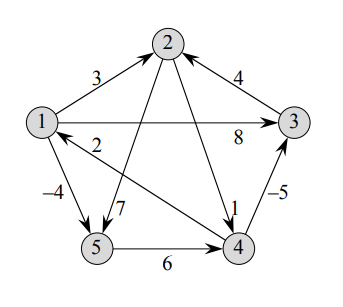
\includegraphics[width=5cm]{graf-25.1}
	\end{subfigure}

	\begin{subfigure}{\linewidth}
	$L^{(1)}=\begin{pmatrix}
		0 & 3 & 8 & \infty & -4\\
		\infty & 0 & \infty & 1 & 7 \\
		\infty & 4 & 0 & \infty & \infty \\
		2 & \infty & -5 & 0 & \infty \\
		\infty & \infty & \infty & 6 & 0
	\end{pmatrix}$
	$L^{(2)}=\begin{pmatrix}
		0 & 3 & 8 & 2 & -4\\
		3 & 0 & -4 & 1 & 7 \\
		\infty & 4 & 0 & 5 & 11 \\
		2 & -1 & -5 & 0 & -2 \\
		8 & \infty & 1 & 6 & 0
	\end{pmatrix}$
	\end{subfigure} \\
	\vspace{0.5cm}
	\begin{subfigure}{\linewidth}
	$L^{(3)}=\begin{pmatrix}
		0 & 3 & -3 & 2 & -4\\
		3 & 0 & -4 & 1 & -1 \\
		7 & 4 & 0 & 5 & 11 \\
		2 & -1 & -5 & 0 & -2 \\
		8 & 5 & 1 & 6 & 0
	\end{pmatrix}$
	$L^{(4)}=\begin{pmatrix}
		0 & 1 & -3 & 2 & -4\\
		3 & 0 & -4 & 1 & -1 \\
		7 & 4 & 0 & 5 & 3 \\
		2 & -1 & -5 & 0 & -2 \\
		8 & 5 & 1 & 6 & 0
	\end{pmatrix}$
	\end{subfigure}
	\caption{Un grafo dirigido y la sucesión de matrices $L^{(m)}$ obtenidas por el proceso recursivo definido en la sección \ref{sec:3.4.1}. La imagen del grafo ha sido extraída de la referencia \cite{algorithms}, capítulo 25, figura 25.1.}
	\label{fig:3.4.1}
\end{figure}

El corazón del algoritmo es el siguiente procedimiento, que, a partir de las matrices $L^{(m-1)}$ y $d$, calcula $L^{(m)}$.

\begin{breakablealgorithm}
	\caption{Extender\_Caminos\_Minimos($L,d$)}
	\begin{algorithmic}[1]
		\State $L'=nueva\ matriz\ n\times n$
		\For{$i=1\ hasta\ n$}
			\For{$j=1\ hasta\ n$}
				\State $l_{ij}'=\infty$
				\For{$k=1\ hasta\ n$}
					\State $l_{ij}'=min(l_{ij}',\ l_{ik}+d_{kj})$
				\EndFor
			\EndFor
		\EndFor
		\Return $L'$
	\end{algorithmic}
\end{breakablealgorithm}

El algoritmo anterior utiliza la matriz $L$ para $L^{(m-1)}$ y devuelve $L'$, que es $L^{(m)}$. \\

A partir de este procedimiento se puede ver la relación entre este algoritmo y la multiplicación de matrices. Supongamos que queremos calcular el producto matricial $C=A\cdot B$ de dos matrices de tamaño $n\times n$. Entonces, para $i,j = 1,...,n$ calcularíamos

$$c_{ij}=\sum_{k=1}^{n}a_{ik}\cdot b_{kj}$$

Realizando las sustituciones

\begin{flalign}
	l^{(m-1)} & \rightarrow a, \\
	d & \rightarrow b, \\
	l^{(m)} & \rightarrow c, \\	
	min & \rightarrow +, \\
	+ & \rightarrow .
\end{flalign}

Podemos transformar la operación de recursión en el producto matricial anterior. Gracias a este hecho, volviendo al problema del cálculo de caminos de longitud mínima, podemos calcular la matriz $L^{(n-1)}$ de la siguiente manera
\begin{adjustwidth}{5cm}{10cm}
\begin{align*}
	L^{(1)} &&=&&  d, \\
	L^{(2)} &&=&&  L^{(1)}\cdot d &&=&& & d^2,\\
	L^{(3)} &&=&&  L^{(2)}\cdot d &&=&& & d^3,\\
	&&&& \vdots \\
	L^{(m-1)} &&=&&  L^{(n-2)}\cdot d &&=&& & d^{n-1}.\\
\end{align*}
\end{adjustwidth}

Podemos calcular este proceso con el siguiente algoritmo

\begin{breakablealgorithm}
	\caption{Caminos\_Minimos\_Todas\_Parejas\_Lento($d$)}
	\begin{algorithmic}[1]
		\State $L^{(1)}=d$
		\For{$m=2\ hasta\ n-1$}
			\State $L^{(m)}=nueva\ matriz\ n\times n$
			\State $L^{(m)}=$Extender\_Caminos\_Minimos($L^{(m-1)},d$)
		\EndFor
		\Return $L^{(n-1)}$
	\end{algorithmic}
\end{breakablealgorithm}

Hemos denotado a este algoritmo como "Lento", pues podemos realizar una mejora muy sencilla que transforma el tiempo de ejecución de este último algoritmo de lineal a logarítmico. Dado que nuestro objetivo es el cálculo de la matriz $L^{(n-1)}$, no nos interesa el cálculo del resto de matrices, por ello, utilizando el hecho de que el algoritmo funciona como el producto de matrices, y que $L^{(m)}=L^{(n-1)}\ \forall m\geq n-1$, podemos calcular $L^{(n-1)}$ de la siguiente manera

\begin{adjustwidth}{3.5cm}{10cm}
	\begin{align*}
		L^{(1)} &&=&&  d, \\
		L^{(2)} &&=&&   d^2 &&=&& & d\cdot d,\\
		L^{(4)} &&=&&   d^4 &&=&&  &d^2\cdot d^2,\\
		L^{(8)} &&=&&   d^8 &&=&&  &d^4\cdot d^4,\\
		&&&& \vdots \\
		L^{(2^{\lceil lg(n-1)\rceil })} &&=&& d^{2^{\lceil lg(n-1)\rceil }} &&=&&  &d^{2^{\lceil lg(n-1)\rceil -1}}\cdot d^{2^{\lceil lg(n-1)\rceil -1}}.\\
	\end{align*}
\end{adjustwidth}

Puesto que $2^{\lceil lg(n-1)\rceil}\geq n-1$ el resultado final es igual a $L^{(n-1)}$. El siguiente algoritmo implementa dicho proceso

\begin{breakablealgorithm}
	\caption{Caminos\_Minimos\_Todas\_Parejas\_Rapido($d$)}
	\begin{algorithmic}[1]
		\State $L^{(1)}=d$
		\State $m=1$
		\While{$m<n-1$}
			\State $L^{(2m)}=nueva\ matriz\ n\times n$
			\State $L^{(2m)}=$Extender\_Caminos\_Minimos($L^{(m)},L^{(m)}$)
			\State $m=2m$
		\EndWhile
		\Return $L^{(m)}$
	\end{algorithmic}
\end{breakablealgorithm}

\subsection{Algoritmo de Floyd-Warshall}

A continuación trataremos el algoritmo de Floyd-Warshall, más eficiente que el algoritmo anterior a la hora de resolver el problema de encontrar los caminos mínimos entre todas las parejas de nodos de un grafo, para ello, el algoritmo considera los vértices intermedios en un camino de longitud mínima, siendo un vértice \textit{intermedio} de un camino simple $p=v_1...v_l$ cualquier vértice a parte de $v_1$ y $v_l$, es decir, cualquier vértice del conjunto $\{v_2,...,v_{l-1}\}$. \\

A partir de este concepto, el algoritmo de Floyd-Warshall se basa en la siguiente observación. Suponiendo que el conjunto de vértices de $G$ son $V=\{1,2,...,n\}$, consideremos un subconjunto $\{1,...,k\}$ de vértices para algún $k$. Para cualquier par de vértices $i,j\in V$ consideremos todos los caminos entre $i$ y $j$ cuyos vértices intermedios están todos en $\{1,...,k\}$, y sea $p$ un camino de longitud mínima entre ellos ($p$ es simple). El algoritmo de Floyd-Warshall utiliza una relación entre $p$ y los caminos entre $i$ y $j$ con todos los vértices intermedios están en el conjunto $\{1,...,k-1\}$. Esta relación depende del hecho de que $k$ sea un vértice intermedio de $p$ o no.

\begin{itemize}
	\item Si $k$ no es un vértice intermedio de $p$, todos los vértices intermedios están en el conjunto $\{1,...,k-1\}$. Entonces, un camino de longitud mínima desde $i$ hasta $j$ con todos los vértices intermedios están en $\{1,...,k-1\}$ es también un camino de longitud mínima desde $i$ hasta $j$ con todos los vértices intermedios en $\{1,...,k\}$.
	\item Si $k$ es un vértice intermedio en $p$, descomponemos $p$ en $i\leadsto^{p_1}k\leadsto^{p_2}j$. Por la \autoref{prop:separa_cam_min_long}, $p_1$ es un camino de longitud mínima entre $i$ y $k$ con todos los vértices intermedios en $\{1,...,k\}$. De hecho, puesto que $k$ no es un vértice intermedio, entonces $p_1$ es un camino de longitud mínima entre $i$ y $k$ con todos los vértices intermedios en $\{1,...,k-1\}$. De la forma similar, $p_2$ es un camino de longitud mínima entre $k$ y $j$ con todos los vértices intermedios en $\{1,...,k-1\}$.
\end{itemize}

A partir de esta observación, se define una fórmula recursiva al igual que se hizo anteriormente. Sea $d_{ij}^{(k)}$ el peso de un camino de longitud mínima entre $i$ y $j$ para el cuál todos sus vértices intermedios están en $\{1,...,k\}$. Cuando $k=0$, los caminos no tienen vértice intermedios, por ello, $d_{ij}^{(0)}=d_{ij}$. Definimos entonces $d_{ij}^{(k)}$ de la siguiente manera

$$d_{ij}^{(k)}= \left\{ \begin{array}{lcc}
	d_{ij} &   si\ k=0, \\
	\\ min(d_{ij}^{(k-1)},\ d_{ik}^{(k-1)}+d_{kj}^{(k-1)}) & si\ k\geq 1.
\end{array}
\right.$$

Puesto que cualquier camino tiene sus vértices intermedios en el conjunto $\{1,...,n\}$, la matriz $D^{(n)}=(d_{ij}^{(n)})$ contiene el resultado final buscado: $d_{ij}^{(n)}=d(i,j)\ \forall i,j\in V.$

\subsubsection{Implementación del algoritmo de Floyd-Warshall}

El pseudocódigo que implementa la recursión descrita anteriormente se muestra a continuación

\begin{breakablealgorithm}
	\caption{Floyd-Warshall($d$)}
	\begin{algorithmic}[1]
		\State $D^{(0)}=d$
		\For{$k=1\ hasta\ n$}
			\State $D^{(k)}=nueva\ matriz\ n\times n$
			\For{$i=1\ hasta\ n$}
				\For{$j=1\ hasta\ n$}
					\State $d_{ij}^{(k)}=min(d_{ij}^{(k-1)},\ d_{ik}^{(k-1)}+d_{kj}^{(k-1)})$
				\EndFor
			\EndFor
		\EndFor
		\Return $D^{(n)}$
	\end{algorithmic}
\end{breakablealgorithm}

Si queremos saber cuáles son los caminos de mínima longitud concretos, podemos calcular la matriz de predecesores $\Pi$ mientras se calculan las matrices $D^{(k)}$. En concreto, calculamos una secuencia de matrices $\Pi^{(0)},\Pi^{(1)},...,\Pi^{(n)}$, donde $\Pi^{(n)}=\Pi$ y $\pi_{ij}^{(k)}$ es el predecesor del vértice $j$ en un camino de longitud mínima desde $i$ con todos los vértices intermedios en el conjunto $\{1,2,...,k\}$. \\

\begin{figure}[!htb]
	\centering
	\begin{subfigure}{\linewidth}
		$D^{(0)}=\begin{pmatrix}
			0 & 3 & 8 & \infty & -4\\
			\infty & 0 & \infty & 1 & 7 \\
			\infty & 4 & 0 & \infty & \infty \\
			2 & \infty & -5 & 0 & \infty \\
			\infty & \infty & \infty & 6 & 0
		\end{pmatrix}$
		$\Pi^{(0)}=\begin{pmatrix}
			NULO & 1 & 1 & NULO & 1\\
			NULO & NULO & NULO & 2 & 2 \\
			NULO & 3 & NULO & NULO & NULO \\
			4 & NULO & 4 & NULO & NULO \\
			NULO & NULO & NULO & 5 & NULO
		\end{pmatrix}$
	\end{subfigure} \\
	\vspace{0.5cm}
	\begin{subfigure}{\linewidth}
		$D^{(1)}=\begin{pmatrix}
			0 & 3 & 8 & \infty & -4\\
			\infty & 0 & \infty & 1 & 7 \\
			\infty & 4 & 0 & \infty & \infty \\
			2 & 5 & -5 & 0 & -2 \\
			\infty & \infty & \infty & 6 & 0
		\end{pmatrix}$
		$\Pi^{(1)}=\begin{pmatrix}
			NULO & 1 & 1 & NULO & 1\\
			NULO & NULO & NULO & 2 & 2 \\
			NULO & 3 & NULO & NULO & NULO \\
			4 & 1 & 4 & NULO & 1 \\
			NULO & NULO & NULO & 5 & NULO
		\end{pmatrix}$
	\end{subfigure} \\
	\vspace{0.5cm}
	\begin{subfigure}{\linewidth}
		$D^{(2)}=\begin{pmatrix}
			0 & 3 & 8 & 4 & -4\\
			\infty & 0 & \infty & 1 & 7 \\
			\infty & 4 & 0 & 5 & 11 \\
			2 & 5 & -5 & 0 & -2 \\
			\infty & \infty & \infty & 6 & 0
		\end{pmatrix}$
		$\Pi^{(2)}=\begin{pmatrix}
			NULO & 1 & 1 & 2 & 1\\
			NULO & NULO & NULO & 2 & 2 \\
			NULO & 3 & NULO & 2 & 2 \\
			4 & 1 & 4 & NULO & 1 \\
			NULO & NULO & NULO & 5 & NULO
		\end{pmatrix}$
	\end{subfigure} \\
	\vspace{0.5cm}
	\begin{subfigure}{\linewidth}
		$D^{(3)}=\begin{pmatrix}
			0 & 3 & 8 & 4 & -4\\
			\infty & 0 & \infty & 1 & 7 \\
			\infty & 4 & 0 & 5 & 11 \\
			2 & -1 & -5 & 0 & -2 \\
			\infty & \infty & \infty & 6 & 0
		\end{pmatrix}$
		$\Pi^{(3)}=\begin{pmatrix}
			NULO & 1 & 1 & 2 & 1\\
			NULO & NULO & NULO & 2 & 2 \\
			NULO & 3 & NULO & 2 & 2 \\
			4 & 3 & 4 & NULO & 1 \\
			NULO & NULO & NULO & 5 & NULO
		\end{pmatrix}$
	\end{subfigure} \\
	\vspace{0.5cm}
	\begin{subfigure}{\linewidth}
		$D^{(4)}=\begin{pmatrix}
			0 & 3 & -1 & 4 & -4\\
			3 & 0 & -4 & 1 & -1 \\
			7 & 4 & 0 & 5 & 3 \\
			2 & -1 & -5 & 0 & -2 \\
			8 & 5 & 1 & 6 & 0
		\end{pmatrix}$
		$\Pi^{(4)}=\begin{pmatrix}
			NULO & 1 & 4 & 2 & 1\\
			4 & NULO & 4 & 2 & 1 \\
			4 & 3 & NULO & 2 & 1 \\
			4 & 3 & 4 & NULO & 1 \\
			4 & 3 & 4 & 5 & NULO
		\end{pmatrix}$
	\end{subfigure} \\
	\vspace{0.5cm}
	\begin{subfigure}{\linewidth}
		$D^{(5)}=\begin{pmatrix}
			0 & 1 & -3 & 2 & -4\\
			3 & 0 & -4 & 1 & -1 \\
			7 & 4 & 0 & 5 & 3 \\
			2 & -1 & -5 & 0 & -2 \\
			8 & 5 & 1 & 6 & 0
		\end{pmatrix}$
		$\Pi^{(5)}=\begin{pmatrix}
			NULO & 3 & 4 & 5 & 1\\
			4 & NULO & 4 & 2 & 1 \\
			4 & 3 & NULO & 2 & 1 \\
			4 & 3 & 4 & NULO & 1 \\
			4 & 3 & 4 & 5 & NULO
		\end{pmatrix}$
	\end{subfigure} \\
	\caption{Secuencia de matrices $D^{(k)}$ y $\Pi^{(k)}$ obtenida a partir del algoritmo de Floyd-Warshall aplicado al grafo de la figura \autoref{fig:3.4.1}}
	\label{fig:3.4.2}
\end{figure}

Para $k=0$, como no hay vértices intermedios, tenemos

$$\pi_{ij}^{(0)}= \left\{ \begin{array}{lcc}
	NULO &   si\ i=j\ o\ d_{ij}=\infty, \\
	\\ i & si\ i\neq j\ y\ d_{ij}<\infty.
\end{array}
\right.$$

Para $k\geq 1$, si al introducir el vértice $k$ hemos creado un camino de longitud menor, escogemos el predecesor de $j$ en un camino de longitud mínima desde $k$, calculado en la iteración $k-1$, si no, nos quedamos con el mismo predecesor que la iteración anterior. Formalmente, 

$$\pi_{ij}^{(k)}= \left\{ \begin{array}{lcc}
	\pi_{ij}^{(k-1)} &   si\ d_{ij}^{(k-1)}\leq d_{ik}^{(k-1)}+d_{kj}^{(k-1)}, \\
	\\ \pi_{kj}^{(k-1)} &   si\ d_{ij}^{(k-1)}> d_{ik}^{(k-1)}+d_{kj}^{(k-1)}.
\end{array}
\right.$$

En la \autoref{fig:3.4.2} podemos observar el resultado de la ejecución del algoritmo sobre un grafo simple. \\

A continuación se muestra el pseudocódigo completo del algoritmo, incluyendo la construcción de la matriz de predecesores

\begin{breakablealgorithm}
	\caption{Floyd-Warshall-Caminos($G,d$)}
	\begin{algorithmic}[1]
		\State $D^{(0)}=d$
		\State $\Pi^{(0)}=nueva\ matriz\ nula\ n\times n$
		\For{$(i,j)\in G.E$}
			\State $\pi_{ij}^{(0)}=i$
		\EndFor
		\For{$k=1\ hasta\ n$}
			\State $D^{(k)},\Pi^{(k)}=nueva\ matriz\ n\times n$
			\For{$i=1\ hasta\ n$}
				\For{$j=1\ hasta\ n$}
					\If{$d_{ij}^{(k-1)}\leq d_{ik}^{(k-1)}+d_{kj}^{(k-1)}$}
						\State $d_{ij}^{(k)}=d_{ij}^{(k-1)}$
						\State $\pi_{ij}^{(k)}=\pi_{ij}^{(k-1)}$
					\Else
						\State $d_{ij}^{(k)}=d_{ik}^{(k-1)}+d_{kj}^{(k-1)}$
						\State $\pi_{ij}^{(k)}=\pi_{kj}^{(k-1)}$
					\EndIf
				\EndFor
			\EndFor
		\EndFor
		\Return $(D^{(n)},\Pi^{(n)})$
	\end{algorithmic}
\end{breakablealgorithm}

\subsubsection{Clausura transitiva de un grafo dirigido}

\begin{definicion}
	Dado un grafo dirigido $G=(V,E)$, se define la \textit{clausura transitiva} de $G$ como el grafo $G^*=(V,E^*)$, donde
	$$E^*=\{(i,j):\ existe\ un\ camino\ desde\ i\ hasta\ j\}.$$
\end{definicion}

La clausura transitiva de un grafo dirigido es muy útil, pues nos permite saber de forma rápida si existe un camino entre dos nodos o no. Para calcularla, basta con asignar peso $1$ a todas las aristas del grafo y ejecutar el algoritmo de FLoyd-Warshall. \\

\begin{figure}[htb]
	\centering
	\begin{subfigure}{\linewidth}
		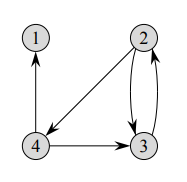
\includegraphics[width=3.5cm]{graf-clausura-transitiva}
	\end{subfigure}
	
	\begin{subfigure}{\linewidth}
		$T^{(0)}=\begin{pmatrix}
			1 & 0 & 0 & 0 &\\
			0 & 1 & 1 & 1 \\
			0 & 1 & 1 & 0 \\
			1 & 0 & 1 & 1 \\
		\end{pmatrix}$
		$T^{(1)}=\begin{pmatrix}
			1 & 0 & 0 & 0 &\\
			0 & 1 & 1 & 1 \\
			0 & 1 & 1 & 0 \\
			1 & 0 & 1 & 1 \\
		\end{pmatrix}$
		$T^{(2)}=\begin{pmatrix}
			1 & 0 & 0 & 0 &\\
			0 & 1 & 1 & 1 \\
			0 & 1 & 1 & 1 \\
			1 & 0 & 1 & 1 \\
		\end{pmatrix}$
	\end{subfigure} \\
	\vspace{0.5cm}
	\begin{subfigure}{\linewidth}
		$T^{(3)}=\begin{pmatrix}
			1 & 0 & 0 & 0 &\\
			0 & 1 & 1 & 1 \\
			0 & 1 & 1 & 1 \\
			1 & 1 & 1 & 1 \\
		\end{pmatrix}$
		$T^{(4)}=\begin{pmatrix}
			1 & 0 & 0 & 0 &\\
			1 & 1 & 1 & 1 \\
			1 & 1 & 1 & 1 \\
			1 & 1 & 1 & 1 \\
		\end{pmatrix}$
	\end{subfigure}
	\caption{Un grafo dirigido y las matrices $T^{(k)}$ calculadas por el algoritmo de la clausura transitiva. La imagen del grafo ha sido extraída de la referencia \cite{algorithms}, capítulo 25, figura 25.5.}
	\label{fig:claus-trans}
\end{figure}

Además, puesto que no necesitamos calcular ningún valor numérico para la clausura transitiva, podemos sustituir los valores numéricos del algoritmo por valores booleanos, es decir, que sólo pueden tomar el valor $0$ ($FALSE$) o $1$ ($TRUE$) y sustituir la operaciones aritméticas por operaciones lógicas. De esta forma podemos ahorrar tiempo y espacio, puesto que las operaciones lógicas son generalmente más rápidas y los valores booleanos ocupan menos espacio. \\

En particular, para aplicar estos cambios, definimos $t_{ij}^{(k)}$ como $1$ si existe un camino entre $i$ y $j$ con vértices intermedios en $\{1,...,k\}$ y $0$ en otro caso. De esta manera podemos construir la clausura transitiva $G^*=(V,E^*)$ añadiendo una arista $(i,j)$ a $E^*$ si $t_{ij}^{(n)}=1$. Para calcular $t_{ij}^{(k)}$ se sigue la siguiente recursión

$$t_{ij}^{(0)}= \left\{ \begin{array}{lcc}
	0 &   si\ i\neq j\ y\ (i,j)\notin E, \\
	\\ 1 & si\ i= j\ o\ (i,j)\in E,
\end{array}
\right.$$

y para $k\geq 1$,

$$t_{ij}^{(k)}=t_{ij}^{(k-1)}\lor (t_{ik}^{(k-1)}\wedge t_{kj}^{(k-1)}).$$ \\

El psuedocódigo que implementa este algoritmo es el siguiente

\begin{breakablealgorithm}
	\caption{Clausura\_Transitiva($G,d$)}
	\begin{algorithmic}[1]
		\State $T^{(0)}=nueva\ matriz\ nula\ n\times n$
		\For{$i=1\ hasta\ n$}
			\For{$j=1\ hasta\ n$}
				\If{$i==j\ or\ (i,j)\in G.E$}
					\State $t_{ij}^{(0)}=1$
				\EndIf
			\EndFor
		\EndFor
		\For{$k=1\ hasta\ n$}
			\State $T^{(k)}=nueva\ matriz\ n\times n$
			\For{$i=1\ hasta\ n$}
				\For{$j=1\ hasta\ n$}
					\State $t_{ij}^{(k)}=t_{ij}^{(k-1)}\lor (t_{ik}^{(k-1)}\wedge t_{kj}^{(k-1)})$
				\EndFor
			\EndFor
		\EndFor
		\Return $T^{(n)}$
	\end{algorithmic}
\end{breakablealgorithm}

Para ilustrar este proceso, en la \autoref{fig:claus-trans} se puede observar el cálculo de las matrices $T^{(k)}$ sobre un grafo arbitrario.



\endinput



